% !root= RH 1.6.tex
\documentclass{article}
\usepackage{tikz}
\usepackage{pgfplots}
\usepackage{setspace}
\usepackage{units}
\usepackage{graphicx}
\usepackage{amsopn}
\usepackage{bbding}
\usepackage{amsmath}
\usepackage{hyperref}
\usepackage{cancel}
\usepackage{etoolbox}
\usepackage{enumitem}
\usepackage{gensymb}
\usepackage{amssymb}
\usepackage{multicol}
\usepackage{numerica}
\usepackage{tikz}
\usetikzlibrary{arrows.meta, calc}
\usepackage[top=0.7in, left=0.8in, right=0.8in, bottom=1in]{geometry}
\AtBeginEnvironment{document}{\everymath{\displaystyle}}
\pagestyle{plain}
\title{RH 1.8}
\author{MATH 5, Jones}
\date{Tejas Patel}
\begin{document}
\maketitle
\section*{Refrigerator Homework}
\subsection*{17}
Since $T$ is linear $T(a\,\mathbf{x}) \;=\;a\,T(\mathbf{x}) \quad\text{and}\quad T(\mathbf{x}+\mathbf{y}) \;=\;T(\mathbf{x})+T(\mathbf{y}).$
\\Given $T(\mathbf{u}) \;=\;\begin{bmatrix}2\\1\end{bmatrix}\quad\text{and}\quad T(\mathbf{v}) \;=\;\begin{bmatrix}-1\\3\end{bmatrix}.$
\\\boxed{3u=3\begin{bmatrix}2\\1\end{bmatrix}= \begin{bmatrix}6\\3\end{bmatrix} \qquad 2v=2\begin{bmatrix}-1\\3\end{bmatrix}= \begin{bmatrix}-2\\6\end{bmatrix} \qquad 3u+2v=\begin{bmatrix}6-2\\3+6\end{bmatrix}=\begin{bmatrix}4\\9\end{bmatrix}}
\subsection*{20}
$\mathbf{e}_1 = \begin{bmatrix}1\\0\end{bmatrix},\quad\mathbf{e}_2 = \begin{bmatrix}0\\1\end{bmatrix}.$\\The first column of A is $T(\mathbf{e}_1)$, and the second column is $T(\mathbf{e}_2)$.\\$T\bigl(x_1,x_2\bigr)=x_1\,v_1 + x_2\,v_2$\\Given that$T(x_1,x_2) \;=\;x_1\,v_{1}\;+\;x_2\,v_{2}$,
then for the standard basis vectors $\mathbf{e}_1=(1,0)$ and $\mathbf{e}_2=(0,1)$ we have$T(\mathbf{e}1) \;=\;v_{1},\quad T(\mathbf{e}2) \;=\;v_{2}$.\\$A \;=\;\bigl[v_{1}\;\;v_{2}\bigr]\;=\;$\boxed{\begin{bmatrix}-2 & 7\\5 & -3\end{bmatrix}}
\subsection*{21}
True. A linear transformation is indeed a function (one that takes vectors as inputs and returns vectors as outputs) but it satisfies two special properties:\\
1.	Additivity: $T(\mathbf{u}+\mathbf{v}) = T(\mathbf{u}) + T(\mathbf{v})$.
\\2.	Homogeneity: $T(c\,\mathbf{u}) = c\,T(\mathbf{u})$ for any scalar c
\\Any function that meets both of these properties is called a linear transformation, so it's a specialized type of function.
\subsection*{24}
False.
The set of all linear combinations of the columns of A is the range (or image) of the transformation function, a subset of its codomain.
When we write $T\colon \mathbb{R}^n \to \mathbb{R}^m$ via $T(\mathbf{x}) = A\mathbf{x}$, the usual codomain is $\mathbb{R}^m$. The range—the set of all possible outputs that T actually attains—coincides with the column space of A. So the column space is a subspace of the codomain, not the entire codomain itself
\subsection*{31}
%------------------------------------------------------------------
% 1) Illustrate  T(u+v) = T(u) + T(v)
%------------------------------------------------------------------
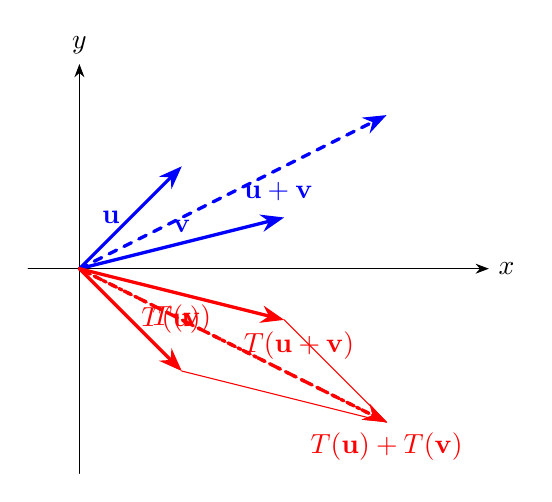
\begin{tikzpicture}[scale=1.3,>=Stealth, line cap=round, line join=round]
    % axes
    \draw[->] (-0.5,0) -- (4,0) node[right] {$x$};
    \draw[->] (0,-2) -- (0,2) node[above] {$y$};
    
    % define vectors u and v (in blue)
    \coordinate (O)   at (0,0);
    \coordinate (u)   at (1,1);
    \coordinate (v)   at (2,0.5);
    \coordinate (u+v) at ($(u)+(v)$);
    
    % reflection across x-axis means (x,y) -> (x,-y)
    \coordinate (Tu)     at ($(u)+(0,-2*1)$);     % reflection of (1,1) is (1,-1)
    \coordinate (Tv)     at ($(v)+(0,-2*0.5)$);   % reflection of (2,0.5) is (2,-0.5)
    \coordinate (Tuv) at ($(u+v) + (0,{-2*1.5})$); % Define the transformed coordinate


    
    %--- draw the original vectors in blue
    \draw[->,very thick,blue]  (O) -- (u)   node[midway,left]  {$\mathbf{u}$};
    \draw[->,very thick,blue]  (O) -- (v)   node[midway,above] {$\mathbf{v}$};
    \draw[->,very thick,blue,dashed] (O) -- (u+v) node[midway,right] {$\mathbf{u}+\mathbf{v}$};
    
    %--- draw the reflected vectors in red
    \draw[->,very thick,red]  (O) -- (Tu)     node[midway,right]  {$T(\mathbf{u})$};
    \draw[->,very thick,red]  (O) -- (Tv)     node[midway,below]  {$T(\mathbf{v})$};
    \draw[->,very thick,red,dashed] (O) -- (Tuv) node[midway,right] {$T(\mathbf{u}+\mathbf{v})$};

    
    %--- show that T(u+v) = T(u) + T(v) by the parallelogram rule
    \draw[thin,red] (Tu) -- ($(Tu)+(Tv)$) -- (Tv);
    \draw[->,very thick,red,dotted] (O) -- ($(Tu)+(Tv)$) node[pos=1,below] {$T(\mathbf{u}) + T(\mathbf{v})$};
    
  \end{tikzpicture}\\
  %------------------------------------------------------------------
  % 2) Illustrate  T(cu) = c T(u)
  %------------------------------------------------------------------
  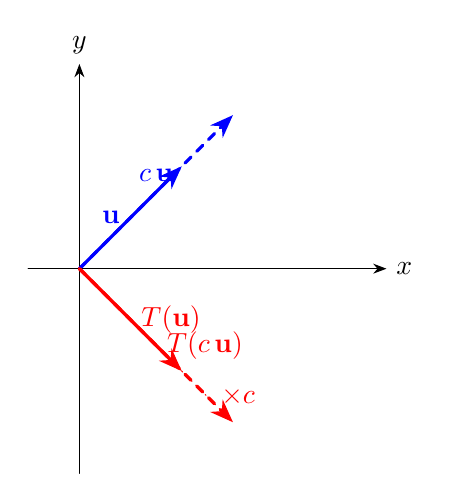
\begin{tikzpicture}[scale=1.3,>=Stealth, line cap=round, line join=round]
    % axes
    \draw[->] (-0.5,0) -- (3,0) node[right] {$x$};
    \draw[->] (0,-2) -- (0,2)  node[above] {$y$};
  
    % pick u = (1,1) and c = 1.5
    \coordinate (O) at (0,0);
    \coordinate (u) at (1,1);
    \def\c{1.5}
    \coordinate (cu) at (\c,\c);
  
    % reflection across x-axis
    \coordinate (Tu)  at (1,-1);
    \coordinate (Tcu) at (\c,-\c);
  
    %--- original vectors in blue
    \draw[->,very thick,blue]        (O) -- (u)  node[midway,left] {$\mathbf{u}$};
    \draw[->,very thick,blue,dashed] (O) -- (cu) node[midway,above] {$c\,\mathbf{u}$};
  
    %--- reflected vectors in red
    \draw[->,very thick,red]        (O) -- (Tu)  node[midway,right] {$T(\mathbf{u})$};
    \draw[->,very thick,red,dashed] (O) -- (Tcu) node[midway,right] {$T(c\,\mathbf{u})$};
  
    % optional guide line to emphasize c*T(u) coincides with T(c*u)
    \draw[dotted,red] (Tu) -- (Tcu);
    \node[red] at ($(Tu)!0.5!(Tcu)+(0.3,0)$) {$\times c$};
  \end{tikzpicture}
\subsection*{32}
1.	Every $\mathbf{x}\in \Bbb R^n$ can be written as a linear combination of the spanning vectors $v_1,\dots,v_p$.  In symbols,

$\mathbf{x} \;=\; c_1\,v_1 \;+\; c_2\,v_2 \;+\;\cdots\;+\;c_p\,v_p.$

	2.	Apply T and use linearity:

$T(\mathbf{x})
\;=\;
T\bigl(c_1\,v_1 + c_2\,v_2 + \cdots + c_p\,v_p\bigr)
\;=\;
c_1\,T(v_1) \;+\; c_2\,T(v_2) \;+\;\cdots\;+\;c_p\,T(v_p)$.

	3.	But each $T(v_i)=\mathbf{0}$, by assumption.  Hence every term on the right is zero, so

$T(\mathbf{x}) = \mathbf{0}$.


Because $\mathbf{x}$ is an arbitrary vector that can span $\mathbb{R}^n$, it follows that $T(\cdot)$ sends every vector to $\mathbf{0}$.
\subsection*{39}
Because $v_1,v_2,v_3$ is dependent, there exist scalars $c_1,c_2,c_3$, not all zero, such that

$c_1\,v_1 \;+\; c_2\,v_2 \;+\; c_3\,v_3 \;=\;\mathbf{0}$.

Apply the linear map T to both sides:

$T\bigl(c_1 v_1 + c_2 v_2 + c_3 v_3\bigr)
\;=\;
c_1\,T(v_1) \;+\; c_2\,T(v_2) \;+\; c_3\,T(v_3)
\;=\;
T(\mathbf{0}) \;=\;\mathbf{0}$.

This shows that

$c_1\,T(v_1) \;+\; c_2\,T(v_2) \;+\; c_3\,T(v_3) \;=\;\mathbf{0}$,

with $(c_1,c_2,c_3)\neq(0,0,0)$, meaning $\,T(v_1),T(v_2),T(v_3)$ is also linearly dependent.
\pagebreak \section*{Computer Homework: Next 10 Pages}
\end{document}
